%!TeX root = application
\documentclass[../main.tex]{subfiles}

\begin{document}
    \section{Flask}    \label{sec:flask}
    Flask is a web application framework written in Python. To be more precise, Flask is a microframework which means it is extensible and is not dependent on third-party library, or, in other word, plug and play. The 

    \pagebreak
    \section{Application's flowchart} \label{sec:application_flowchart}
    The following diagram is the application's flowchart.
    \begin{figure}[!h]
        \centerline{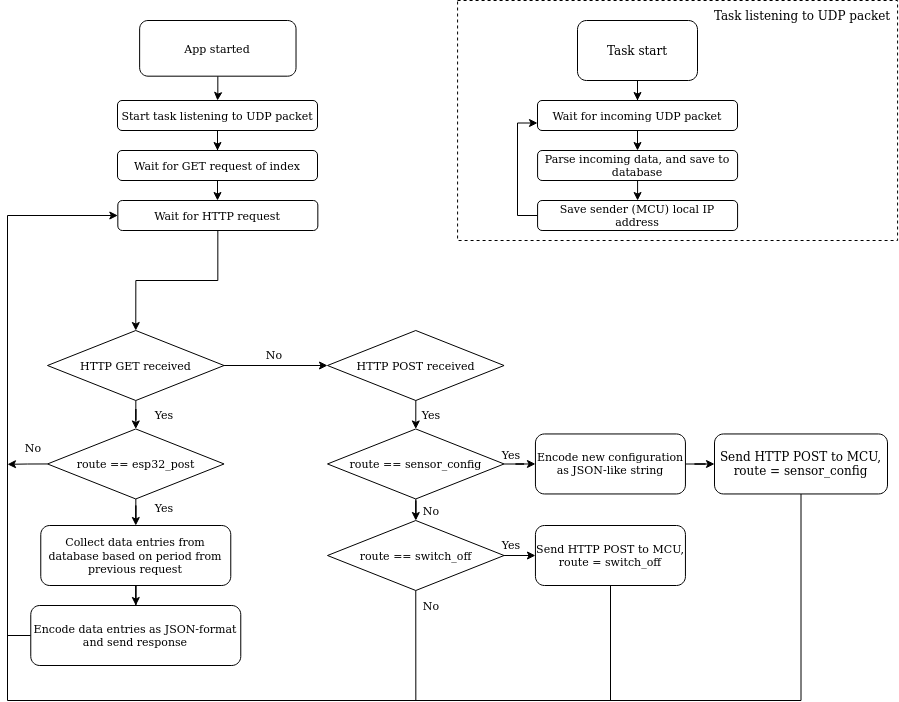
\includegraphics[scale=0.5]{media/appliation_flowchart.drawio.png}}
        \caption{Application's flowchart.}
        \label{fig:application_flowchart}
    \end{figure}

    \justify
    \begin{itemize} 
        \item An asynchronous task reading incoming UDP packets is started with the application. The asynchronous task parses and saves the incoming data to the database. The sender (MCU)'s local IP address is also stored for other operation.
        \item The web application can then be accessed in the preferred browser with the host PC/laptop's local IP adress at port 8090.
        \item The first GET request is for acquiring the html of the main page.
        \item A GET request with requested resource "esp\_post" is sent every 1000ms from client to the host. The response includes all the data entries from the previous request time up until now. Thus, no data entries sent by the MCU will not be missed.
        \item Other POST requests are "redirected" to the MCU with similar route discussed in previous section.
    \end{itemize}
\end{document}